% Fig. 3.17 -- 條件版全機率定理的兩張積分範圍對照 (兩面板)。
% 書稿來源: mathstatch3.tex 第 2603 至 2641 行 (左面板) 與第 2645 至 2685 行 (右面板)，
%   兩個 tikzpicture 同在一個 center 之內、各放一個 .45\textwidth 的 minipage 並排，
%   依 CH3_FIGURE_SPECS.md 第二節併為一張兩面板的圖。
% 書稿以 gray、opacity 0.2 填色, 網頁改 journalaccent、透明度 0.15。
%
% 對書稿原圖的兩處刻意改正 (比照 Fig. 3.1 的既有處置, 併入勘誤登錄):
%   一、書稿兩面板的實線都畫到超出 x=1 與 y=1 所界定的方形之外 (左面板到 (1.6, 3.2)、
%       右面板到 (3.1, 1.55))，網頁把線收在方形的邊上, 標示改掛在交點旁。
%   二、書稿把面板下方的 z 範圍寫成行內 \frac，分子分母會被降到 script 級；
%       網頁改用 \dfrac，分子分母與其餘標示同為 12pt (CH2_FIGURE_SPECS.md 1.3)。
%
% 字級: 全圖標示一律 \large (12pt)，圖內沒有下標、指數與行內分數，
%   最小的一級即 12pt。原生寬度見產圖後的量測。
\documentclass[tikz,border=2pt]{standalone}
\usepackage{amsmath}
\usepackage{amssymb}
\usepackage{xcolor}

\definecolor{journalink}{HTML}{1F1C18}
\definecolor{journalmuted}{HTML}{8A7F72}
\definecolor{journalaccent}{HTML}{9C2D2D}

\begin{document}
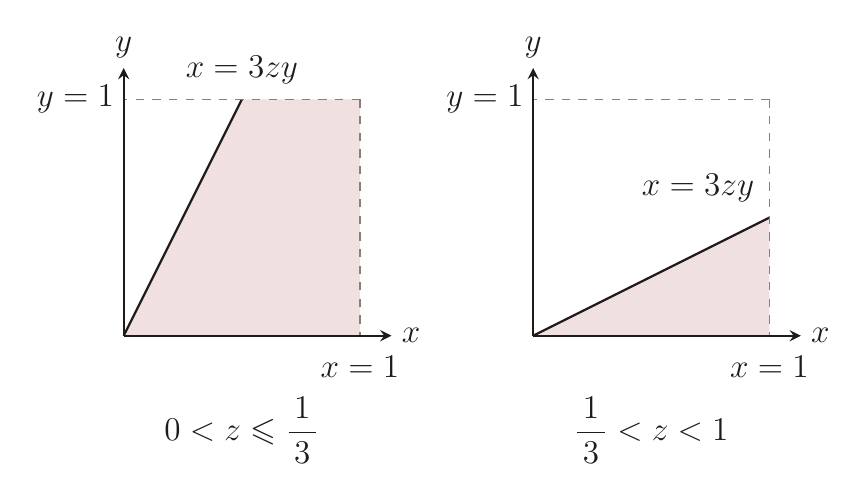
\begin{tikzpicture}[x=1cm, y=1cm, >=stealth,
                    every node/.style={journalink, font=\large}]

  %% 面板共用的部分: 兩條虛線界出 x=1 與 y=1，兩軸帶箭頭
  \newcommand{\panelframe}{%
    \draw[journalmuted, line width=0.5pt, dashed] (3,3) -- (3,0);
    \node[below, yshift=-4pt] at (3,0) {$x=1$};
    \draw[journalmuted, line width=0.5pt, dashed] (3,3) -- (0,3);
    \node[left] at (0,3) {$y=1$};
    \draw[journalink, line width=0.8pt, ->] (0,0) -- (3.4,0) node[right] {$x$};
    \draw[journalink, line width=0.8pt, ->] (0,0) -- (0,3.4) node[above] {$y$};
  }

  %% ---- 左面板: 直線與方形的上邊相交，填色的部分是四邊形 ----
  \begin{scope}[shift={(0,0)}]
    \fill[journalaccent, fill opacity=0.15]
      (0,0) -- (1.5,3) -- (3,3) -- (3,0) -- cycle;
    \draw[journalink, line width=0.8pt] (0,0) -- (1.5,3);
    \node[above, yshift=2pt] at (1.5,3) {$x=3zy$};
    \panelframe
    \node at (1.5,-1.2) {$0<z\leqslant\dfrac{1}{\,3\,}$};
  \end{scope}

  %% ---- 右面板: 直線與方形的右邊相交，填色的部分是三角形 ----
  \begin{scope}[shift={(5.2,0)}]
    \fill[journalaccent, fill opacity=0.15]
      (0,0) -- (3,1.5) -- (3,0) -- cycle;
    \draw[journalink, line width=0.8pt] (0,0) -- (3,1.5);
    \node[above left, xshift=-2pt, yshift=2pt] at (3,1.5) {$x=3zy$};
    \panelframe
    \node at (1.5,-1.2) {$\dfrac{1}{\,3\,}<z<1$};
  \end{scope}

\end{tikzpicture}
\end{document}
